\documentclass[a4paper, 12pt]{article}

% packages
\usepackage{natbib}
\usepackage[english]{babel}
\usepackage{fancyhdr}
\usepackage{setspace}
\usepackage{longtable}
\usepackage{parskip}
\usepackage[hidelinks]{hyperref}
\usepackage{xfrac}
\usepackage{fontspec} 
\usepackage[margin=1.2in]{geometry}
\usepackage{booktabs}
\usepackage[section]{placeins}
\setmainfont{Times New Roman}

\newcommand\addrow[2]{#1 &#2\\ }

\newcommand\addheading[2]{#1 &#2\\ \hline}
\newcommand\tabularhead{\begin{tabular}{lp{8cm}}
\hline
}

\newcommand\addmulrow[2]{ \begin{minipage}[t][][t]{2.5cm}#1\end{minipage}% 
   &\begin{minipage}[t][][t]{8cm}
    \begin{enumerate} #2   \end{enumerate}
    \end{minipage}\\ }

\newenvironment{usecase}{\tabularhead}
{\hline\end{tabular}}


\begin{document}

\doublespacing

\begin{abstract}

Motion analysis has been a research area that has been widely studied by the computer vision community over the past decade. Human motion analysis involves the use of special computer vision devices for tracking, detecting and recognising humans and understanding human behaviour from image sequences captured using these computer vision devices. This has led to further research into how these devices can be used for motion analysis for health-related problems (e.g. injuries). The Vicon 3D is a powerful system that has been used extensively for motion capture, analysis and estimation. Although powerful, it is very expensive to purchase, difficult to install. Moreover, it requires patients to wear additional equipment and highly trained staff to operate the equipment. As a result, a cheaper alternative is required for applications which do not require such complex systems. 
The Microsoft Kinect sensor is a low-cost device which is capable of generating 3D image and video frames and tracking human movements. Furthermore, it is easy to install and setup and contains software development kits (SDKs) which can be used to develop programs for motion analysis. This project seeks to develop a user-friendly application help medical professionals analyse the progress of recovery made by injured patients. This will be achieved by analysing the movements made by the upper limbs of the patient.

\end{abstract}

\newpage


\renewcommand{\abstractname}{Acknowledgements}
\begin{abstract}
I would like to acknowledge Dr Charles Day for his guidance, advice, support and feedback for all my deliverables for this module. Additionally, I will like to thank my family and loved ones for their tremendous support and encouragement throughout this academic year.
\end{abstract}

\newpage

\tableofcontents

\newpage

\section{Introduction}

\subsection{Problem Statement}

Motion analysis has been a major research topic and has been applied to many applications in various areas such as medicine, gaming, sports science and robotics.  In the medical field, motion analysis has been particularly useful for diagnosing health problems such as Parkinson’s disease \citep{Galnaetal2014} and monitoring the recovery of patients. By studying and analysing quantified data provided from the movements of the limbs of patients, medical professionals are able to determine the how well a patient is recovering and will be able to determine or plan out the next course of action during therapy. Additionally, diagnosis for certain movement or gait disorders can be done easily by carefully studying the results obtained from the data. \citet{Mireketal2007} achieve this by using the Vicon three-dimensional motion analysis system to assess gait disorders in patients with Parkinson’s disease. Although the Vicon system is very accurate, it is an expensive system to purchase, install and maintain, moreover it requires highly trained staff and this adds to the economic burden. Therefore, there is a need for a fast and simple method to quantify limb movements of a patient accurately but at a low cost. 

\subsection{Purpose of project}

The need to be able to quantify movement in the upper limb, for example when reporting the severity of impairment or monitoring the progress of recovery is of rising importance. Advanced systems for 3D motion analysis such as Vicon are available, but a fast, simple and low-cost means of doing this accurately has yet to be developed. The Microsoft Kinect has the ability to record 3D points as well as track a virtual skeleton and has been proven to provide a decent level of accuracy \citep{Clarketal2012}\citep{Galnaetal2014}. Therefore, it is a plausible solution to this problem. This project seeks to design a user-friendly interface that will allow a clinician to record arm movements and be presented with data such as range of motion, movement speed etc. This will be achieved using the Java programming language and the J4K Library developed by \citet{barmpoutis2013} and Microsoft's Kinect Studio.

\subsection{Project Aim and Objectives}

\subsubsection{Aim}
Developing a user-friendly software to quantify movement in the upper limb of patients and using the data to help user to understand the progress of recovery.

\subsubsection{Objectives}

\begin{itemize}
	\item Identify the ability of motion tracking on Kinect.
	\item Quantify movement of the upper limb.
	\item Allow patient to see the performance of the upper limb.
	\item Allow user to record data of patient’s movement in video and text.
	\item Allow user to compare data of patient’s movement.
\end{itemize}

\newpage

\subsection{Background and Related Work}

According to \citet{Microsoft2018}, the Kinect sensor has 25 joints per person to complete skeleton. The Kinect sensor also has the ability to capture motion and video frames at a rate of 30 frames per second. Additionally, the Kinect provides enough data for low velocity motions such as griping an apple or waving hands in the air. \citet{Parajulietal2012} suggested a system to monitor the health of elderly individuals by analysing their gait and posture changes as their posture changed from sitting to standing and vice versa. Gait and posture changes were analysed using data recorded by the Kinect sensor. Before 2013, the Kinect sensor only had 20 joints to shape the skeletons, however recent developments in the sensor's technology has led to the ability to track positions more accurately and autonomously. An experiment which assessed the abilities of Microsoft Kinect and Vicon 3D motion capture for gait analysis, was done by \citet{Pfisteretal2014}. The experiment involved tracking the movements of individuals at three separate velocities while walking or jogging on a treadmill and featured 20 healthy adults. The results from stride timing measurements and concurrent hip and knee peak flexion and extension and were juxtaposed between Vicon and Kinect. Regardless of the fact that the Kinect measurements were indicative of normal gait, the Kinect sensor under-emphasised joint flexion and exaggerated extension \citep{Pfisteretal2014}.The data produced by the Kinect and Vicon for hip angular displacement correlation was very low with a large error. However, results obtained for knee measurements using the Kinect were relatively more desirable than that of hip angular displacement, nonetheless, the results were not stable enough for clinical assessment \citep{Pfisteretal2014}. In addition, correlation between Kinect and Vicon stride timing was high and the magnitude of errors produced were rather small. Therefore from the experiments, it was concluded that the Kinect will be an adequate device for measuring stride timing after some minor adjustments, however in order to meet the requirements for clinical use,  the Kinect sensor will need more powerful hardware and additional software.  


\section{Requirements Definition}

This section discusses how the requirements were defined and obtained in order to develop the application to aid in progress monitoring in the upper limbs of patients. The prototyping software development life cycle was used to develop the application. Two main prototypes were developed over the course of this project. This section contains the requirements for the first prototype. The revised requirements for the next prototype will be discussed in the subsequent sections.

\subsection{Basic Requirement Identification}
This was the first stage of the application development process. This involved obtaining a basic understanding of the fundamental requirements of the client. A meeting was arranged with the client in order to determine these requirements. According to \citet{Sabale2012}, this is usually in terms of user interface, however in this case since it was the beginning of the project, the look and feel of the graphical user interface was not really clear.

The initial requirement stated by the client was to: 
\begin{itemize}
 \item Show movements of the upper limbs with data
\end{itemize} 

How the data was represented was left to be determined by the developer to decide. After the basic requirement was identified, the next step was to define the application requirements for the first prototype. A few more meetings were arranged with the client in order to ensure that the requirements were clearly defined. The requirements that were defined from the meetings can be found in the objectives section (section 1.3.2) of this report. 



\subsection{Application Requirements}
Application requirements can be broken down into two categories. These are function requirements and non-functional requirements. Function requirements are the necessary tasks or processes that must be completed therefore, functional requirements are defined in terms of what needs to be carried out \citep{Defence2001}. Non functional requirements serve as constraints on the services of function that the system provides. These include factors such as reliability, portability, ease of use etc. Eide (2005) explains constraints as restrictions on the software engineering process or factors which affect the processes of the life cycle. Disregarded constraints may have negative implications on the developed system. The functional and non-functional requirements for the application prototype stated in tables one and two. 

\begin{table}[!htb]
 \centering
 \textbf{\caption{Functional Requirements}}
 \begin{tabular}{|c|}
  \hline
   Display video footage from WebCam and Kinect sensor \\
  \hline 
   Provide means of recording patient data as text and video stream \\
  \hline
   Provide means of comparing recorded data of patient's movement  \\
  \hline
   Provide functionality to load recorded data back into system \\
   \hline
   Quantify movement of upper limbs of patient \\
   \hline
   Calculate speed of movement and height of movement \\
  \hline
 \end{tabular}
\end{table}


\begin{table}[!htb]
 \centering
 \textbf{\caption{Non-Functional Requirements}}
 \begin{tabular}{| c | c |}
 \hline
  Non-Functional Requirement & Requirement Metric\\
  \hline
   Ease of Use & Length of training time \\
  \hline 
   Reliability &  Rate of failure occurrence  \\
  \hline
   Robustness & Probability of data corruption after system fails malfunction \\
  \hline
   Speed & Response time to user events \\
  \hline
 \end{tabular}
\end{table}

The functional requirements were documented using use case descriptions. The reason for using use case descriptions can be found in the section below.  

\subsection{Use Case Descriptions}
Use cases are defined by  Jackobson et al. (2011) as the methods used by an end user to achieve a specific task or goal. The purpose of using use cases is to understand completely how the system works and the different ways in which the system can be used. This helps with the development process because, the use cases present a logical explanation of how the system should work.
\parskip 0.2in

The Use case descriptions for the first prototype can be seen below:

\begin{usecase}
	\addheading{Name of Use Case}{Starting the application}
	\addrow{ID}{1}
	\addrow{Actor}{End User}
	\addrow{Description}{This describes the necessary steps needed to start the application}
	\addrow{Pre-Condition}{The Application must be installed on the user's computer.}
	\addmulrow{Successful Completion}{
		\item User navigates to location of executable file. 
		\item User clicks executable file. 
		\item The application opens up.}
	\addmulrow{Alternatives}{
	\item Java not installed on system. 
	\item Kinect cannot be detected or is not plugged in.}
	\addmulrow{Assumptions}{
	\item Kinect is connected to computer. 
	\item Application is installed.}
\end{usecase}

\begin{usecase}
	\addheading{Name of Use Case}{Obtaining video footage from WebCam}
	\addrow{ID}{2}
	\addrow{Actor}{Application}
	\addrow{Description}{This describes how video footage is obtained from the web camera}
	\addrow{Pre-Condition}{Computer must be connected to a web camera}
	\addmulrow{Successful Completion}{
		\item User clicks on the execute button. 
		\item The application open up a window with four main panels. 
		\item Thread which handles WebCam initialisation starts
		\item The WebCam initialisation thread completes. 
		\item Thread that handles showing the video footage starts.
		\item The camera footage is displayed at the top left panel of user interface.}
	\addmulrow{Alternatives}{
	\item Webcam cannot be detected by the application.
	\item Application is already running.}
	\addmulrow{Assumptions}{
	\item Webcam is connected to the computer. 
	\item Application is installed.}
\end{usecase}

\begin{usecase}
	\addheading{Name of Use Case}{Obtaining video footage from Kinect sensor}
	\addrow{ID}{3}
	\addrow{Actor}{Application}
	\addrow{Description}{This describes how video footage is obtained from the Kinect sensor}
	\addrow{Pre-Condition}{Kinect sensor must be connected to the computer}
	\addmulrow{Successful Completion}{
		\item User clicks on the execute button. 
		\item The application opens up a window with four main panels. 
		\item Thread which handles kinect initialisation starts
		\item The initialisation thread completes. 
		\item Three new threads which handle the depth, color and skeletal display are initiated.
		\item The video footage obtained from the Kinect sensor is displayed at the top right panel of user interface.}
	\addmulrow{Alternatives}{
	\item Kinect sensor cannot be detected by the application although plugged in
	\item Kinect sensor is not plugged into the computer}
	\addmulrow{Assumptions}{
	\item Kinect sensor is connected to the computer.
	\item Kinect sensor is detected by application 
	\item Application is installed.}
\end{usecase}

\begin{usecase}
	\addheading{Name of Use Case}{Displaying coordinate positions of limbs in table}
	\addrow{ID}{4}
	\addrow{Actor}{User and Application}
	\addrow{Description}{This describes how the coordinate positions (x and y) values are obtained using the Kinect sensor and displayed in a table.}
	\addrow{Pre-Condition}{Kinect sensor must be connected to the computer}
	\addmulrow{Successful Completion}{
		\item User opens the Application
		\item The application opens up a window with four main panels. 
		\item Application displays video footage from WebCam and Kinect sensor.
		\item Kinect sensor detects patient.  
		\item Skeleton is projected on Kinect video stream.
		\item Application extracts X and Y coordinates recorded by the Kinect sensor as limbs move.  
		\item The application then shows the recorded data in table displayed at the bottom left panel of the interface.}
	\addmulrow{Alternatives}{
	\item Kinect sensor cannot be detected by the application although plugged in
	\item Kinect sensor cannot detect patient and project skeleton on Kinect video stream}
	\addmulrow{Assumptions}{
	\item Kinect sensor is detected by application 
	\item Seated skeleton tracking is enabled}
\end{usecase}


\begin{usecase}
	\addheading{Name of Use Case}{Start recording data from Kinect sensor}
	\addrow{ID}{5}
	\addrow{Actor}{End User}
	\addrow{Description}{This describes the necessary steps to start obtaining data from Kinect sensor}
	\addrow{Pre-Condition}{The Kinect Sensor must be plugged in.}
	\addmulrow{Successful Completion}{
		\item User selects the start button displayed on the user interface. 
		\item A panel showing the length of the recording along with other controls is displayed on screen.
		\item the user selects the record button.
		\item The Kinect sensor begins capturing the data. 
		\item X and Y coordinates of upper limbs displayed in a table on user interface.}
	\addmulrow{Alternatives}{ 
	\item Kinect cannot be detected or is not plugged in.
	\item User positioned too close to Kinect, hence Kinect cannot detect skeleton.}
	\addmulrow{Assumptions}{
	\item Kinect is connected to computer. 
	\item User skeleton is detected.}
\end{usecase}

\begin{usecase}
	\addheading{Name of Use Case}{Stop Recording Data from Kinect Sensor}
	\addrow{ID}{6}
	\addrow{Actor}{End User}
	\addrow{Description}{This describes how video data being recorded is stopped.}
	\addrow{Pre-Condition}{The Application must be recording live data (video and text).}
	\addmulrow{Successful Completion}{
		\item User selects the stop button displayed on the control panel. 
		\item the Kinect sensor stops capturing data.
		\item The data showing coordinates of patient limbs (text) stops displaying in the table. 
		\item The skeleton disappears from the screen.}
	\addmulrow{Alternatives}{ 
	\item The Kinect sensor loses power and turns off.}
	\addmulrow{Assumptions}{
	\item Kinect sensor never turns off. 
	\item The application is already recording.}
\end{usecase}

\begin{usecase}
	\addheading{Name of Use Case}{Save recorded data from Kinect sensor as text }
	\addrow{ID}{7}
	\addrow{Actor}{End User}
	\addrow{Description}{Describes how data obtained from Kinect sensor is saved as text.}
	\addrow{Pre-Condition}{The Application must be recording or have recorded live data.}
	\addmulrow{Successful Completion}{
		\item User clicks on the save button displayed on the control panel. 
		\item A dialog box displays on screen with a file chooser. 
		\item User selects the path to where the data is to be saved.
		\item The data is saved at location specified by the user in a csv file.
		\item Message box displays message "Data Saved Successfully"}
	\addmulrow{Alternatives}{ 
	\item The data does not save after save button is clicked.
	\item file is corrupted during save operation.}
	\addmulrow{Assumptions}{
	\item Kinect sensor never turns off. }
\end{usecase}

\begin{usecase}
	\addheading{Name of Use Case}{Save recorded data from Kinect sensor in video format }
	\addrow{ID}{8}
	\addrow{Actor}{End User}
	\addrow{Description}{Describes how data obtained from Kinect sensor is saved in video format.}
	\addrow{Pre-Condition}{The Application must be recording or have recorded live data.}
	\addmulrow{Successful Completion}{
		\item User selects "File" and then "Save as" from external panel. 
		\item A dialog box displays on screen with a file chooser. 
		\item User selects the path to where the data is to be saved.
		\item The data is saved at location specified by the user as a video.}
	\addmulrow{Alternatives}{ 
	\item The data does not save after save button is clicked 
	\item file is corrupted during save operation.}
	\addmulrow{Assumptions}{
	\item Kinect sensor never turns off. }
\end{usecase}

\begin{usecase}
	\addheading{Name of Use Case}{Load recorded movement data by Kinect sensor as text }
	\addrow{ID}{9}
	\addrow{Actor}{End User}
	\addrow{Description}{Describes how coordinate data stored as text is loaded into a table.}
	\addrow{Pre-Condition}{The saved file must exist and should contain coordinate data .}
	\addmulrow{Successful Completion}{
		\item User clicks on the load button displayed on the control panel. 
		\item A dialog box displays on screen with a file chooser. 
		\item User selects the path to where the saved csv file stored.
		\item The data saved at location specified is loaded into the application.
		\item The loaded data is displayed in a table on the bottom right corner of the screen.}
	\addmulrow{Alternatives}{ 
	\item The saved file cannot be found or does not exist 
	\item file cannot be loaded because it is corrupted.}
	\addmulrow{Assumptions}{
	\item The saved file exists on the system 
	\item The data is never corrupted}
\end{usecase}


\begin{usecase}
	\addheading{Name of Use Case}{Comparing old saved data with live data}
	\addrow{ID}{10}
	\addrow{Actor}{End User}
	\addrow{Description}{This describes how the old data can be compared with live data by displaying both old and live data simultaneously.}
	\addmulrow{Pre-Condition}{
	\item The Application must be recording live data (video and text).
	\item Coordinate data must have been saved in the csv file.}							
	\addmulrow{Successful Completion}{
		\item User selects the load button displayed on the control panel. 
		\item A dialog box pops up with a file chooser for user to select path of saved file.
		\item User selects the saved file from the specified path. 
		\item Data is loaded into a table displayed on the user interface
		\item User selects start button to begin recording
		\item Kinect starts recording coordinate data obtained from skeleton and video footage.
		\item User selects stop button
		\item Kinect stops recording data. 
		\item Both new data and old data are displayed in tables.}
	\addmulrow{Assumptions}{
	\item Kinect sensor never turns off. 
	\item The saved data is never corrupted.
	\item The Kinect sensor detects the patient}
\end{usecase}


\begin{usecase}
	\addheading{Name of Use Case}{Quitting the application}
	\addrow{ID}{11}
	\addrow{Actor}{End User}
	\addrow{Description}{This describes the necessary steps needed to close the application}
	\addrow{Pre-Condition}{The Application must be running}
	\addmulrow{Successful Completion}{
		\item User clicks on close button on the window frame. 
		\item Application displays dialogue box asking if the user wants to quit.  
		\item The user selects yes.
		\item The application closes.}
	\addmulrow{Alternatives}{
	\item The user selects no on the dialogue box. 
	\item The application keeps running.}
	\addmulrow{Assumptions}{
	\item The application is already running. 
	\item The application closes when the user selects yes on dialogue box.}
\end{usecase}




\subsection{Data Gathering}
After the requirements were defined, the next step was to gather data pertaining to the motion of the upper limbs. This data was gathered using the Kinect sensor. The Kinect sensor was connected to a dedicated computer and the Kinect development toolkit was used to test whether the Kinect sensor was functioning properly. A simple Java program was written using the J4K library to extract the skeletal coordinates (X and Y positions) of the upper limbs for simple actions such as lifting the arm to a certain height and waving the arm. 


\section{Application Design} 

This section discusses the design of the first, second and third prototypes including any design decisions that were made during the design process. 

\subsection{Choice of Development Methodology}

Before selecting the development methodology, a comparison was done between known existing methodology to determine the best methodology for the project. Some methodologies that were considered were the waterfall model, incremental model and the rapid application development model \citep{Sabale2012}. The waterfall is a simple model were development stages are clearly defined. The waterfall model was not chosen because, it is most suitable for projects where requirements have been clearly defined at the start of the project. However this project does not have clearly defined requirements at the beginning. Furthermore, the waterfall model only involves users at the beginning of the project meaning that the user is not involved throughout the lifetime of the project. This is not desirable because the end product may be different from the user's expectations.  Using the Rapid application development model as the development methodology seemed plausible as it is suitable for situations where the requirements are easily understood and it is a simple model to implement, however similar to the waterfall model, user involvement is only at the beginning of the project and this may affect the success of the project. With the incremental model, requirements are well understood at the beginning of the project. Additionally, it is relatively simple to implement and is most suitable for very long projects \citep{Sabale2012}. The problem with the incremental model is that, it requires high expertise and has relatively low user involvement.

\parskip 0.2in

After careful consideration of the development models, the prototyping model was chosen as the development methodology for this project. This is because, the prototyping model prioritises the development of the actual application rather than documentation. Furthermore, the prototyping model allows for more user involvement and therefore prevents any misunderstandings that could occur between the client and the developer. As a result, the final product developed will be more desirable as any requirement changes desired by the user will have been satisfied \citep{Sabale2012}.


\subsection{Choice of Development Language}
Microsoft provide a very good software development toolkit which requires writing programs in the $C\#$ programming language. This was an important factor to consider because although the $C\#$ language is relatively easy to learn, a better alternative was to use the Java programming language. This is because, Java was the language that was taught throughout the degree and therefore, it was much easier to use for development than $C\#$ as $C\#$ had to be learnt. Furthermore, Java had libraries for manipulating the Kinect which were relatively well documented and easy to use. 

\subsection{Choice of Development Library for Kinect}

After carrying out research on available development libraries for the Kinect sensor, three main libraries were found and their strengths and weaknesses were compared and contrasted. These three libraries were: 

\begin{itemize}
	\item Java for Kinect (J4K)
	\item Open NI
	\item Open Kinect
\end{itemize}

\subsubsection{Open Kinect}
Open Kinect is an open source library with a large community of developers consisting of individuals interested in using the Kinect sensor for the development of applications on platforms such as Windows, Mac OS and Linux (OpenKinect, 2012). Although the Open Kinect library contains all the necessary functions to use for this project and has wrappers to enable programming in the Java programming language, it was very challenging to configure and required to be compiled first using the CMake library before use. Additionally, the documentation provided was very sparse and quite challenging to understand. 

\subsubsection{Open NI SDK}

The Open NI software development kit similar to Open Kinect is an open source SDK which is used for the development of three dimensional sensing applications. It is also supported and maintained by a wide range of developers (OpenNI, 2018). Unlike the Open Kinect the Open NI SDK has an API documentation which explains the class names, methods etc. The only problem with this SDK is that, the API is documented in the$C++$ language, moreover it was also quite difficult to configure and hence was not the best option to use. 
 
\subsubsection{Java For Kinect (J4K)}
The Java for Kinect Library (J4K) is a well known open source library which contains a Java binding to the Microsoft Kinect SDK. The Kinect library is compatible with the available Kinect devices and enables the control of multiple sensors within an application (University of Florida Digital Worlds Institute, 2013). The J4K library is relatively well documented as API documentation is provided for the 4 main API classes (J4KSDK, DepthMap, Skeleton and VideoFrame). Furthermore, it contains well explained examples showing how the classes can be used. 

The Java for Kinect library was chosen because, it was already integrated with the Java programming language, moreover, the API documentation was simple and easy to understand and examples were available to demonstrate how the various classes could be used.

\subsection{Design of first prototype}
The initial prototype was a simple model that was designed to show the user the look and feel of the graphical user interface. As a result, it contained no implementation. In order to design a user-friendly graphical user interface,  a few factors had to be taken into consideration. These factors were: 

\begin{itemize}
	\item An intuitive and consistent design
	\item Clarity of user interface
	\item Attractiveness of user interface
	\item Accessibility (e.g. colour blindness) 
	\item Simplicity
\end{itemize}


With these factors in mind, the user interface was designed using wire frames before implementing a runnable user interface using the Java Swing library.

\subsubsection{The Application Screen}

In designing the main screen, the screen layout was an important factor to consider (Martin, 1996). Since it was required that the application shows video footage from both the Webcam and Kinect sensor, a good layout was to place these two side by side horizontally. Furthermore, it was required that the user be able to view movement data as text. It was decided to show this data using a table. This is because tables are a simple and intuitive way of organising data and moreover, tables make comparisons between data easy because of the way the data is organised. Therefore the user interface was separated into four main panels. The first panel was used to display the Webcam footage whilst the second and third panels were used to display the Kinect video stream and the movement data respectively. A fourth panel was used to show a log of recorded data however, this was changed in the subsequent prototypes. The four panel layout made the GUI simple and intuitive as the function of each panel was distinguishable (i.e. Kinect Panel shows Kinect stream, Data panel shows movement data etc.). The wireframe of the application screen can be seen in Figure 1 below. The next stage of the design of the application screen was to determine where to place the control panels to start and stop recording video footages and to save or load data respectively. Building on from the first wire frame, the best position to place the recording panel (with start start, stop and pause buttons) was under the kinect panel. Similarly the save and load control panel was placed under the data panel. This was done in order to keep the design consistent and for easy access to the control panels. The complete GUI can be seen in Figure 2.  


\begin{figure}
  \begin{center}
  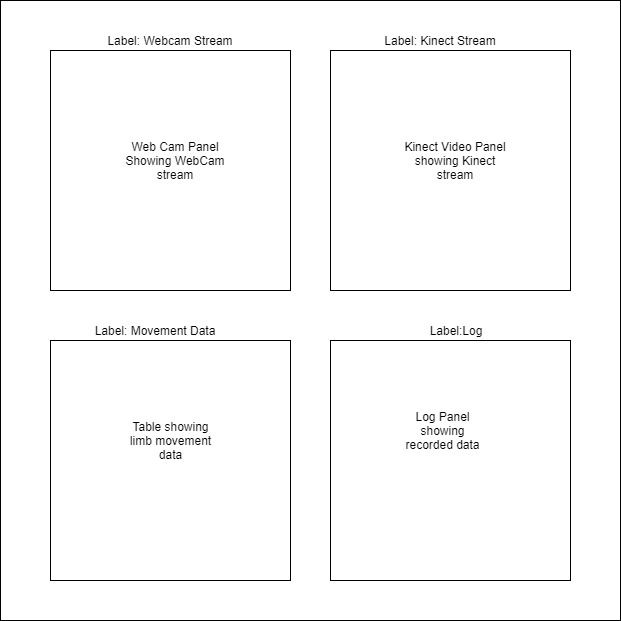
\includegraphics[scale=0.7]{appgui.jpg}
  	\caption{Wireframe of Main Application window.}
  \end{center} 
  \label{fig:appgui} 
\end{figure}

\begin{figure}
  \begin{center}
  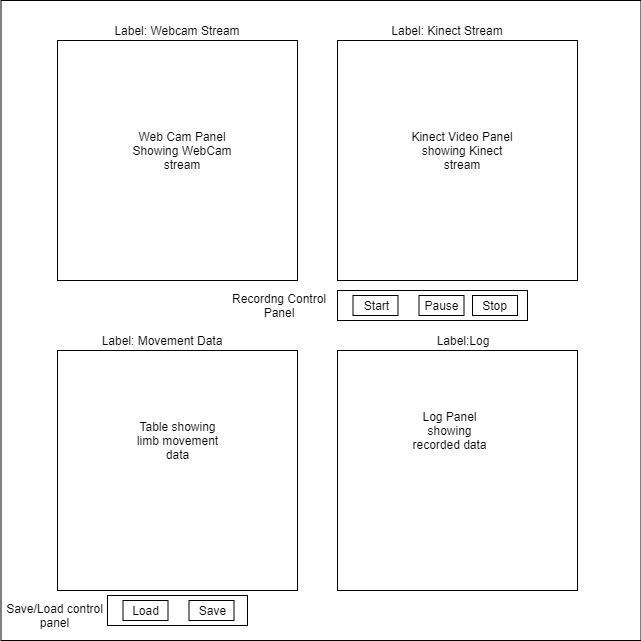
\includegraphics[scale=0.7]{appgui2.jpg}
  	\caption{Wireframe of Main Application window with control panels.}
  \end{center} 
  \label{fig:appgui2} 
\end{figure}

\newpage
\newpage
 
\subsection{Design of second prototype}
The second prototype was an improvement of the first prototype with implementation added to the graphical user interface to create a working program, however without the ability to save movement data as text or video. Before writing any program code, the main classes that were essential for the development of the application were identified. The main were identified from the use case descriptions and were documented using unified modelling language (UML). The Kinect and ViewerPanel3D classes were obtained from the J4K library developed by University of Florida Digital Institute (2013). 


\begin{table}[!htb]
 \centering
 \textbf{\caption{MyTableData Class}}
 \begin{tabular}{|c|}
  \hline
   MyTableData \\
  \hline
   - bodyPart: String  \\
   - xPos: float \\
   - yPos: float \\
  \hline
   + MyTableData(String bodyPart, float xPos, float yPos) \\
   + setBodyPart(String type) \\
   + setxPos(): void \\
   + setyPos (): void \\
   + getBodyPart(): void \\
   + getXPos(): void \\
   + getYPos(): void \\
   + toString(): void \\
   \hline
 \end{tabular}
\end{table}


\begin{table}[!htb]
 \centering
 \textbf{\caption{TableModel Class}}
 \begin{tabular}{|c|}
  \hline
   TableModel \\
  \hline
   - tableData: ArrayList  \\
   - columnName: String[] \\
  \hline
   + TableModel() \\
   + getColumnCount() \\
   + getColumnName(): String \\
   + getRowCount (): int \\
   + getBodyPart(): void \\
   + deleteData(): void \\
   + getValueAt(): Object \\
   + getTableData(): ArrayList \\
   \hline
 \end{tabular}
\end{table}



\begin{table}
 \centering
 \textbf{\caption{Kinect Class}}
 \begin{tabular}{|c|}
  \hline
   Kinect \\
  \hline
   - viewer: ViewerPanel3D  \\
   - label: JLabel \\
   - maskPlayers: boolean \\
   - tableModel: TableModel \\
  \hline
   + Kinect() \\
   + Kinect(byte type) \\
   + setViewer(): void \\
   + setLabel (): void \\
   + onColorFrameEvent(): void \\
   + onSkeletonFrameEvent(): void \\
   + onDepthFrameEvent(): void \\
   + onInfraredFrameEvent(): void \\
   + updateTexturesUsingInfrared(): void \\
   + getTableModel(): TableModel \\
   \hline
 \end{tabular}
\end{table}


\begin{table}
 \centering
 \textbf{\caption{ViewerPanel3D Class}}
 \begin{tabular}{|c|}
  \hline 
   ViewerPanel3D \\
  \hline
   - xRotation: float \\
   - yRotation: float \\
   - zRotation: float \\
   - mouseX : int \\
   - mouseY : int \\
   - isVideoPlaying: boolean \\
   - showVideo: boolean \\
   \textasciitilde skeletons[]: Skeleton \\
   \textasciitilde map: DepthMap \\
   \textasciitilde videoTexture: VideoFrame \\
  \hline
   + setup(): void \\
   + draw(): void \\
   + mousePressed(): void \\
   + mouseClicked(): void \\
   + setShowVideo(boolean flag): void\\
   \hline
 \end{tabular}
\end{table}

\newpage 

\begin{table}
 \centering
 \textbf{\caption{KinectApp Class}}
 \begin{tabular}{|c|}
  \hline
   Kinect App \\
  \hline
   - dataPanel: JPanel \\
   - logPanel: JPanel \\
   - logContorls: JPanel \\
   - lblWebCamStream : JLabel \\
   - lblKinectStream : JLabel \\
   - lblLiveData : JLabel \\
   - lblLogPanel : JLabel \\ 
   - dataControlPanel: JPanel \\
   - btnLoad : Jbutton \\
   - btnSave : Jbutton \\
   - btnStart : Jbutton \\
   - btnPause : Jbutton \\
   - btnStop : Jbutton \\
   - btnClear : Jbutton \\
   - messageFrame: JFrame \\
   - fileChooser : JFileChooser \\
   - csvReader: Scanner \\
   - comboBox : JComboBox \\
   \textasciitilde myKinect: Kinect \\
   \textasciitilde viewer: ViewerPanel3D \\
   \textasciitilde accelerometer: JLabel \\
  \hline
   + getKinect(): Kinect \\
   + getComboSelectedValue(): int \\
   + main(String[] args): void \\
   \hline
 \end{tabular}
\end{table}

\subsubsection{Class Diagram}
Figure 3 shows the class diagram which is depicts the structure of the application to be developed. The purpose of using the class diagram is to show the classes of the system and the various relationships that exist between the classes. Each of the classes have attributes or fields and methods which perform specific functions. The class diagram aided in the understanding of how the classes are linked together and this made the implementation stage much easier. 

\begin{figure}[!htb]
	\begin{center}
  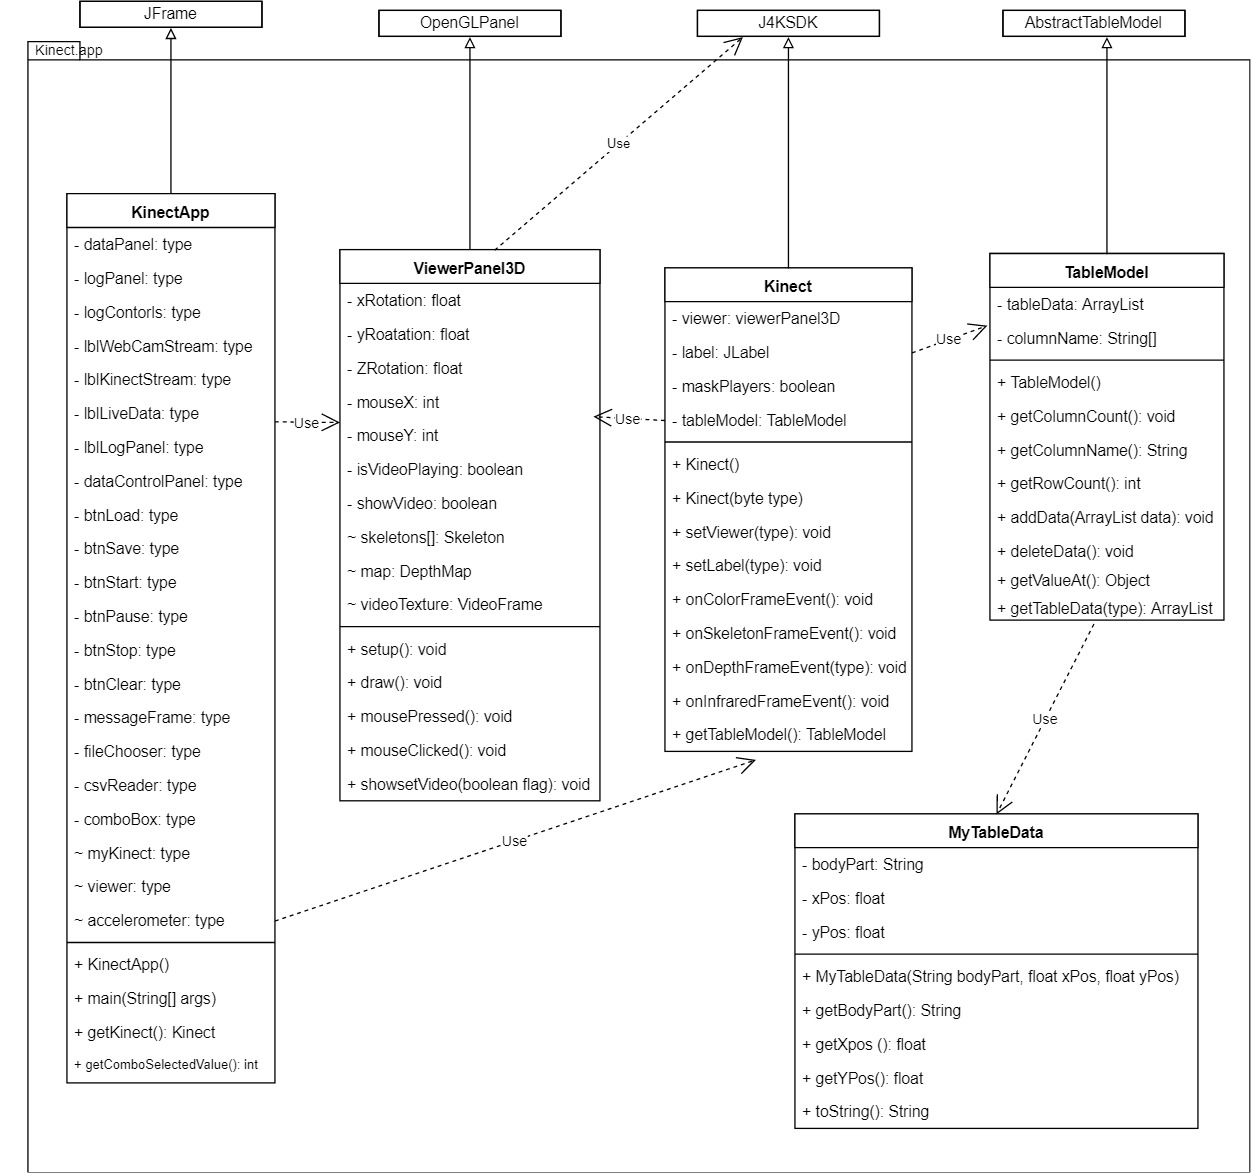
\includegraphics[scale=0.4]{classdiagram.jpg}
  	\caption{Class diagram showing inheritance and dependency between classes.}
  \end{center} 
  \label{fig: classDiagram} 
\end{figure}



\subsubsection{Explanation of dependencies}
The 5 main classes (i.e. Kinect, ViewerPanel3D, TableModel, KinectApp, MyTableData) are all contained within the kinect.app package and are sub classes of the J4K class, OpenGL class, AbstractDataModel class and JFrame class. The MyTableData class is an exception and does not inherit attributes from any of the other classes stated above. The start point of the system resides in the main method of the KinectApp class. The KinectApp class depends on both the Kinect class and the ViewerPanel3D class. The KinectApp class uses an instance of the Kinect class to initialise the Kinect sensor. The ViewerPanel3D handles the rendering of frames obtained from the Kinect sensor. Furthermore, the Kinect class depends on the Viewer3DPanel class. The reason being that, the Kinect class requires frames obtained from the Viewer3DPanel class in order to execute the four methods (onColorFrameEvent(), onSkeletonFrameEvent(), onDepthFrameEvent() and onInfraredFrameEvent() ). The Kinect class also uses or depends on the TableModel class. This is because, the Kinect class makes use of a Table model object to carry out some functions. This will be explained in further detail in the implementation section. Additionally, the TableModel class depends on the MyTableData class because, the TableModel requires data in order to perform its functions and this data is obtained from the MyTableData class.

\subsection{Design of third prototype}

The third prototype was the final prototype that was designed. It contained all of the functionality of the second prototype however, minor changes were made to the graphical user interface including the ability to save movement data in both video and text formats. From figure 1 in section 3.4.1, the fourth panel contained a log which showed where the save recordings were. This was changed to a table which showed old movement data loaded from a CSV file. Also the functions for saving and loading data live data movement data captured as text were implemented in this prototype.

\begin{figure}[!htb]
	\begin{center}
  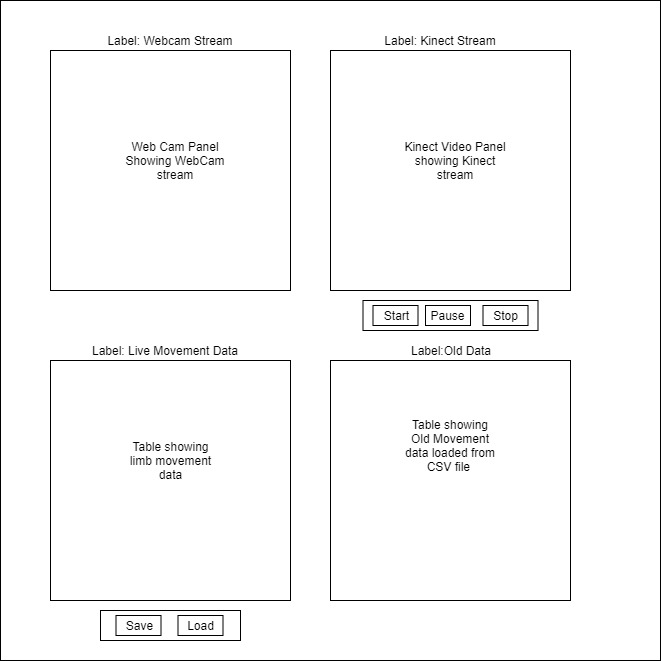
\includegraphics[scale=0.7]{3PrototypeUI.jpg}
  	\caption{Wireframe of the third prototype.}
  \end{center} 
  \label{fig: 3rdPrototype} 
\end{figure}

\clearpage
\newpage 

\section{Application Development}
This section explains how the application was implemented and includes some snippets of code. The designs that were discussed in the section above were used for the implementation of the application. The libraries that were used for the development of the application were: 

\begin{itemize}
 \item Java for Kinect Library - Capturing data from Kinect sensor.
 \item Java Swing Library - For building graphical user interface.
 \item Webcam capture Library - Displaying video footage obtained from WebCam
 \item JOGL library - Rendering frames obtained from Kinect Sensor.  
\end{itemize}


\subsection{Implementation of first prototype}

This prototype was only meant to give the user an idea of the general look and feel of the application and therefore contained no implementation of events such as mouse and button clicks. The following snippets of code reveal how the panels used in the GUI were created along with some additional components such as the main application window frame and table.  

The first step was to create the main application window. This was done by creating the KinectApp class and making it a subclass of the JFrame class and thus, inheriting the methods of the JFrame class. This made it possible to use methods for setting the Layout manager along with settings such as the frame size, position on the screen etc. in the constructor of the KinectApp class. This can be seen in the code snippet below. 

\begin{figure}[!htb]
	\begin{center}
  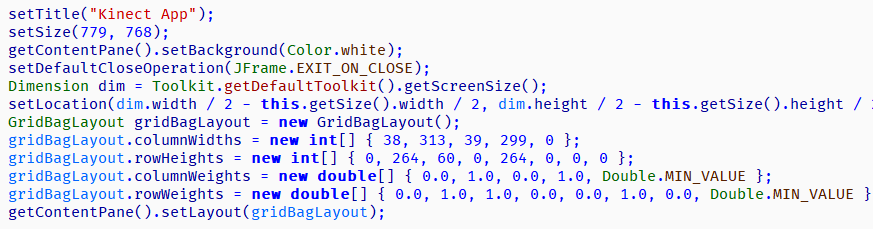
\includegraphics[scale=0.7]{codesnippet5.png}
  	\caption{Code snippet showing how the main application frame was created.}
  \end{center} 
  \label{fig: codesnippet1} 
\end{figure}

The layout manager that was used to ensure that the graphical user interface was arranged appropriately was the Grid Bag Layout. The Grid Bag Layout manager is one of the most resilient and intricate layout managers provided by the Swing class (Oracle, 2017). Grid Bag Layout was used because it is one of the most flexible layout managers and secondly, the use of a grid makes it easy to visualise how components are positioned on the frame. The Grid Bag Constraints (GBC) is used to position the component on the grid and add spaces between components (done by the insets() method). Similar source code was used for the creation of the other three panels (for more detailed code see appendix). 

\begin{figure}[!htb]
	\begin{center}
  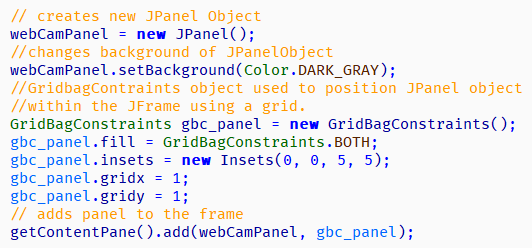
\includegraphics[scale=0.7]{codesnippet1.png}
  	\caption{Creating WebCam Panel.}
  \end{center} 
  \label{fig: codesnippet2} 
\end{figure}


After the creation of the four panels, the next step was to add the control panels and buttons to the controls panels. The control panels were created using code similar to what is seen in figure 6. The buttons were added to their respective panels using the add() method of the JPanel class. This simply adds any JComponent object (in this case buttons) to the panel. 


\begin{figure}[!htb]
	\begin{center}
  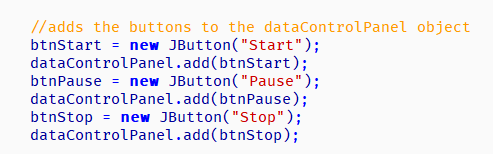
\includegraphics[scale=0.7]{codesnippet3.png}
  	\caption{Adding buttons to the control panels.}
  \end{center} 
  \label{fig: codesnippet3} 
\end{figure}

After the buttons were added to the control panels the final step was to create the table which displayed live movement data from the Kinect sensor stream. In order to add data and display data from a table, a table model is required. The creation of the TableModel class is described in the section below. The table model is accessed using an instance of the Kinect class and is added to the table using the setModel() method of the JTable class. This can be seen in the code snippet below. 

\begin{figure}[!htb]
	\begin{center}
  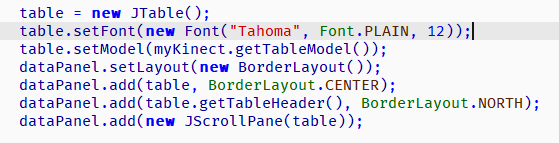
\includegraphics[scale=0.7]{codesnippet4.png}
  	\caption{ Table generation.}
  \end{center} 
  \label{fig: codesnippet4} 
\end{figure}

\subsection{Implementation of second prototype}

As stated in the design section, the second prototype was an improvement of the first prototype and included the implementation of classes and events. At this stage, the first step was to create the 4 classes described in the class diagram and in the tables in section 3.5. Code snippets are shown for the main methods of each class (for more program code pertaining to implementation see appendix).

\subsubsection{The Kinect Class}

The Kinect class extended the J4KSDK abstract class. This required the implementation of three main methods. That is the : 

\begin{itemize}
 \item onDepthFrameEvent()
 \item onColorFrameEvent()
 \item onSkeletonFrameEvent()
\end{itemize}  

These three methods are callback functions and are called whenever a color frame, a depth frame and a skeleton frame is obtained from the Kinect sensor. The implementation of these methods were obtained University of Florida Digital Worlds Institute (2013) with some minor changes. The implementations can be seen in the code snippets below: 

\begin{figure}[!htb]
	\begin{center}
  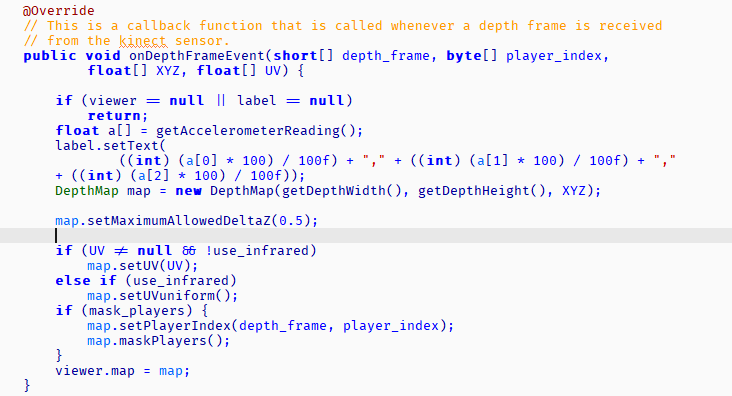
\includegraphics[scale=0.75]{codesnippet6.png}
  	\caption{implemetation of onDepthFrameEvent() method.}
  \end{center} 
  \label{fig: codesnippet5} 
\end{figure}

The method first checks to see if an instance of the ViewerPanel3D exists or if an instance of the label exists. If not, the method returns to the function body of the calling function. If a UV texture exists and the boolean flag $use\_infrared$ is set to true, then the the depth map is set to that UV texture. On the other hand, if a UV texture does not exist, then then a uniform UV texture is generated for the depth map. The ViewerPanel3D's depth map is then set to the generated depth map. 

\begin{figure}[!htb]
	\begin{center}
  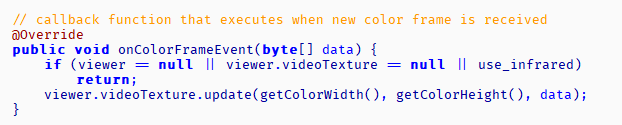
\includegraphics[scale=0.75]{codesnippet7.png}
  	\caption{implemetation of onColorFrameEvent() method.}
  \end{center} 
  \label{fig: codesnippet6} 
\end{figure}

This callback function is a simple call back function which executes when a new color frame is received. If there is no instance of the ViewerPanel3D or a video texture frame or the flag to use infrared is set to false, then the function returns to the body of the calling function, otherwise, the ViewerPanel3D is updated with the new video texture frame.

\begin{figure}[!htb]
	\begin{center}
  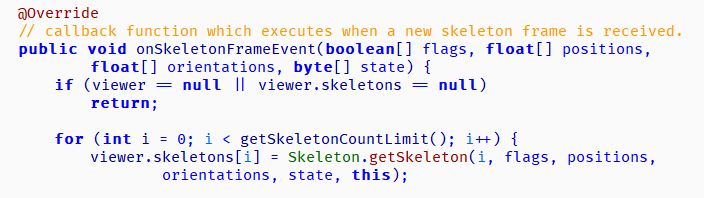
\includegraphics[scale=0.75]{codesnippet8.png}
  	\caption{implemetation of onSkeletonFrameEvent() method.}
  \end{center} 
  \label{fig: codesnippet7} 
\end{figure}

Similar to the two callback methods explained above, this callback method also checks to see if an instance of the ViewerPanel3D exists or if a skeleton frame exists. If both exist then on each skeleton frame, the ViewerPanel3D object is updated with the position and orientation of the skeleton from the received skeleton frame.  

\subsubsection{The TableModel class}

The purpose of the TableModel class was to act as a data model for the JTable object used in the KinectApp class. The TableModel class was a subclass of the AbstractTableModel class and therefore similar to the Kinect class, the TableModel class had to implement 3 main methods which were: 

\begin{itemize}
 \item getColumnCount()
 \item getRowCount()
 \item getValueAt()
\end{itemize} 

before explaining how these methods were implemented it is important to explain the constructor of the TableModel class. The constructor of the TableModel class was a simple one it only created an ArrayList. The purpose of this array list was to hold data to be used by the TableModel class (see appendix for full code). The getColumnCount() method obtains the number of columns defined from a string array. The getRowCount() method gets the number of rows equal to the size of the arrayList. The getValueAt() method updates the contents of the each cell in the table based on the table row index. This row index is passed to the get() method of the ArrayList class to retrieve the necessary information for that row. Code snippets for these methods can be seen below: 

\begin{figure}[!htb]
	\begin{center}
  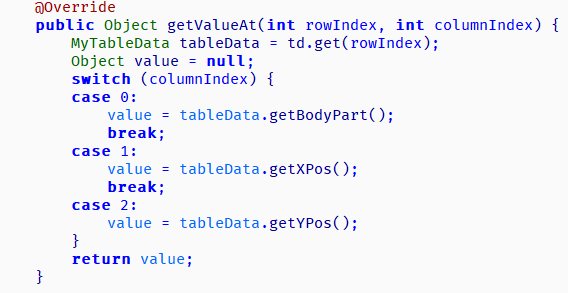
\includegraphics[scale=0.9]{codesnippet10.png}
  	\caption{implemetation of getValueAt() method.}
  \end{center} 
  \label{fig: codesnippet9} 
\end{figure}

\begin{figure}[!htb]
	\begin{center}
  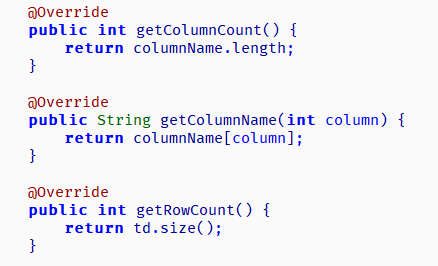
\includegraphics[scale=0.75]{codesnippet9.png}
  	\caption{implemetation of getColumnCount() and getRowCount() methods.}
  \end{center} 
  \label{fig: codesnippet8} 
\end{figure}


\subsubsection{MyTableData class}

The purpose of the MyTableData class was to be able to provide a custom data type to the TableModel class. This is because an ArrayList only takes a single parameter (Object type) and therefore there was a need to create a custom class to enable the user of 3 parameters i.e. (bodyPart, Xpos and yPos). The main methods are the constructor, accessor methods and the toString() method. 

\begin{figure}[!htb]
	\begin{center}
  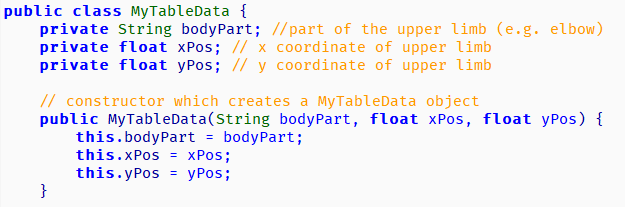
\includegraphics[scale=1.0]{codesnippet11.png}
  	\caption{implemetation of constructor method}
  \end{center} 
  \label{fig: codesnippet10} 
\end{figure}

\begin{figure}[!htb]
	\begin{center}
  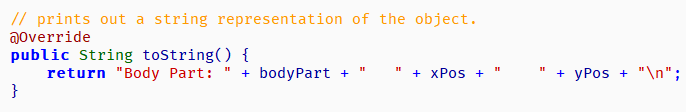
\includegraphics[scale=0.9]{codesnippet13.png}
  	\caption{implemetation of toString() method.}
  \end{center} 
  \label{fig: codesnippet12} 
\end{figure}

\begin{figure}
	\begin{center}
  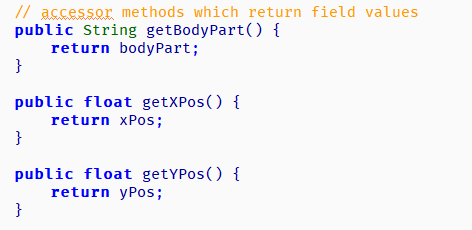
\includegraphics[scale=0.9]{codesnippet12.png}
  	\caption{implemetation of accessor methods.}
  \end{center} 
  \label{fig: codesnippet11} 
\end{figure}


After this the next step was to implement the mouse click events for the start, pause and stop methods. This was done by first adding a MouseListener and overriding the mouseClicked method. 

\subsubsection{Implementation of Button Events}

The start button was implemented such that, it called an external program Kinect Studio which was installed on the $C:$ drive of the computer. This Kinect Studio application was used to record the video footage and playback the recorded footage. The Kinect Studio application searches for a running application using the Kinect sensor and then connects to that application. 

\begin{figure}[!htb]
	\begin{center}
  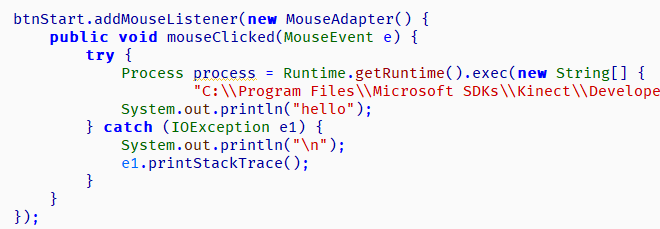
\includegraphics[scale=0.7]{codesnippet14.png}
  	\caption{implemetation of start button.}
  \end{center} 
  \label{fig: codesnippet13} 
\end{figure}

The implementation of the pause button and stop buttons were very simple. When the pause button was clicked, the stop() method is called to stop capturing video frames from the Kinect sensor (same for stop button) and the button text is set to unpause. When the pause button is clicked again, the ViewerPanel3D object is reinitialised. 

\begin{figure}[!htb]
	\begin{center}
  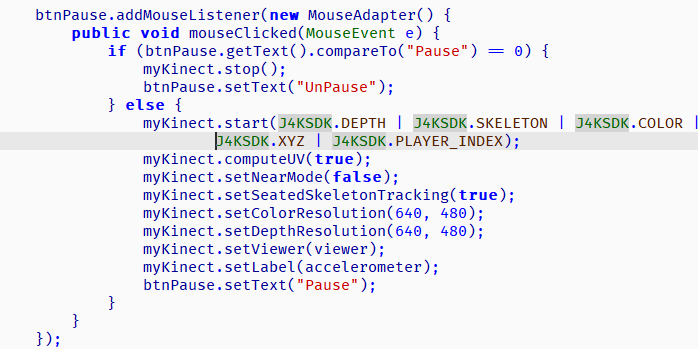
\includegraphics[scale=0.7]{codesnippet15.png}
  	\caption{implemetation of pause button.}
  \end{center} 
  \label{fig: codesnippet14} 
\end{figure}

\begin{figure}[!htb]
	\begin{center}
  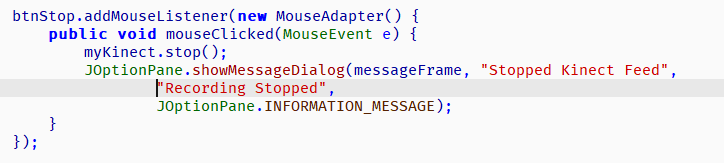
\includegraphics[scale=0.7]{codesnippet16.png}
  	\caption{implemetation of stop button.}
  \end{center} 
  \label{fig: codesnippet15} 
\end{figure}

For implementation of the ViewerPanel3D class see appendix.

\subsection{Implementation of third prototype}

After a requirements evaluation, it was raised that there should be functionality to save and load movement data as text and video. This functionality was added in the third prototype along with replacing the log panel with a table showing old data loaded from a csv file  (see figure 8 for table creation code).

The load button was implemented based on the use case describing how movement data is loaded as text into a table (secton 2.3 use case 8). The implementation of the load function is shown in figure 20. 

\begin{figure}[!htb]
	\begin{center}
  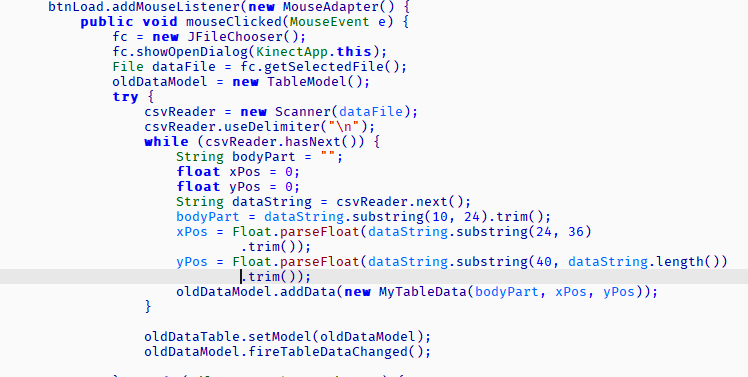
\includegraphics[scale=0.8]{codesnippet18.png}
  	\caption{implemetation of load button.}
  \end{center} 
  \label{fig: codesnippet17} 
\end{figure}

A data model is created for the table and the old movement data is loaded using a Scanner object. The loaded data is parsed and then added to and the parsed data is used to create a MyTableData object. This object is then passed to the addData() method (see TableModel class in appendix) of the TableModel object  and the data is added to the table.

 \begin{figure}[!htb]
	\begin{center}
  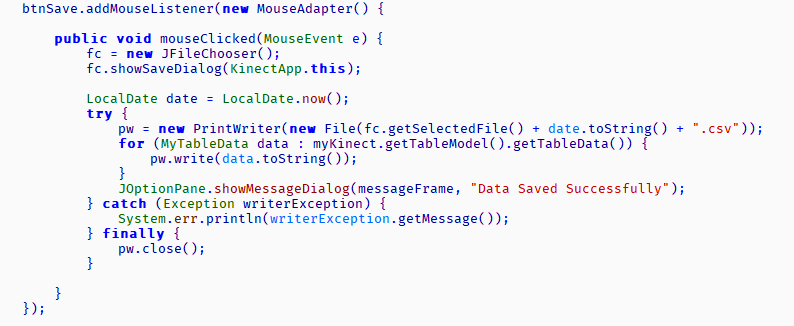
\includegraphics[scale=0.75]{codesnippet17.png}
  	\caption{implemetation of save button.}
  \end{center} 
  \label{fig: codesnippet16} 
\end{figure}

Similarly the save button was implemented based on the use case describing how movement data is saved as text (section 2.3 use case 7). Figure 21 above shows how this was implemented. A PrintWriter object is used to write the data to the file. The ArrayList holding the table data is iterated over and the data is converted to a string format using the toString() method.

The Kinect studio application was used to save and load data recorded in video format. As explained earlier, the Kinect studio application connects to an application instance using the Kinect sensor. This
made it possible to save, load and playback recorded videos in the ViewerPanel3D of the KinectApp class.   

\section{Testing of Application}

The purpose of application testing is to confirm whether the developed application meets the requirements defined at the requirements stage and to ensure that the software satisfies the reasons for its intended use (Ammann and Offutt , 2017). This section is broken down into three sub-sections which explain how the three prototypes were tested and what type of testing was done. 

\subsection{Testing the first prototype}

The type of testing that was done for the first prototype was usability testing. The reason for using usability testing was because the first prototype was only a graphical user interface, thus usability testing was done to assess the usefulness of the user interface. 

\newpage
The graphical user interface was tested against five main criteria as suggested by (Rubin and Chisnell , 2008).


\begin{table}[!htb]
 \centering
 \textbf{\caption{Explanation of usability testing criteria}}
 \begin{tabular}{|c|c|}
 \hline
  Criteria & Explanation \\
  \hline
   Accessibility & Does the application consider individuals with disabilities?  \\
  \hline 
   Efficiency & How quick does the application allow users to accomplish goals?  \\
  \hline
   Effectiveness & Does the application function according to the expectations of the user?  \\
  \hline
   Learnability & Does the user use the application with ease over a short period of time?  \\
  \hline
   Usefulness & To what degree does the application allow users to complete tasks?  \\
  \hline
 \end{tabular}
 \end{table}


\subsection{Testing the second prototype}

Since the second prototype was an implementation of the functions required by the application, the type of testing that was carried out was functional testing. Functional testing as described by Myers (2004) is the process of testing the application against the stated requirements at the start of the project. 

This section shows the test cases along with the results from the test. The execution steps for each test were obtained from the use case descriptions in the requirements section. 

\begin{table}[!htb]
 \begin{tabular}{|p{4cm}|p{10cm}|}
 \hline
  TestCase Field & Details \\
  \hline
   Test Case ID:1 & Starting the application  \\
  \hline 
   Purpose & To determine whether the application loads without any errors  \\
  \hline
   Initiation Criteria & The user selects the application executable to start the application  \\
  \hline
   Execution Steps & See successful completion of use case with ID 1.  \\
  \hline
   Expected results & The application should load main screen without any errors.  \\
  \hline
 \end{tabular}
\end{table}

\begin{table}[!htb]
 \begin{tabular}{|p{4cm}|p{10cm}|}
 \hline
  TestCase Field & Details \\
  \hline
   Test Case ID:2 & Obtaining video footage from Webcam.  \\
  \hline 
   Purpose & To determine video footage could be captured successfully by the WebCam.  \\
  \hline
   Initiation Criteria & When the application executable is clicked, the application initialises Webcam and shows footage in Webcam Panel.  \\
  \hline
   Execution Steps & See successful completion of use case with ID 2.  \\
  \hline
   Expected results & Live video stream should be shown in the Webcam panel.  \\
  \hline
 \end{tabular}
 \end{table}
 
\begin{table}[!htb]
 \begin{tabular}{|p{4cm}|p{10cm}|}
 \hline
  TestCase Field & Details \\
  \hline
   Test Case ID:3 & Obtaining video footage from Kinect sensor.  \\
  \hline 
   Purpose & To determine video footage could be captured successfully from Kinect sensor.  \\
  \hline
   Initiation Criteria & When the application executable is clicked, the application initialises Kinect sensor and shows video stream in Kinect panel.  \\
  \hline
   Execution Steps & See successful completion of use case with ID 3.  \\
  \hline
   Expected results & Live video stream  obtained from Kinect should be shown in Kinect panel.  \\
  \hline
 \end{tabular}
\end{table}
 
 
\begin{table}[!htb]
 \begin{tabular}{|p{4cm}|p{10cm}|}
 \hline
  TestCase Field & Details \\
  \hline
   Test Case ID:4 & Displaying coordinate positions of limbs in table.  \\
  \hline 
   Purpose & To determine the coordinate positions of the limbs are obtained and displayed in a table.  \\
  \hline
   Initiation Criteria & When a Video Frame is obtained from Kinect sensor, X and Y coordinates are extracted from Skeleton data and displayed in a table. \\
  \hline
   Execution Steps & See successful completion of use case with ID 4.  \\
  \hline
   Expected results & X and Y coordinates for each part of the limb(Wrist, Elbow and Shoulder) should be displayed in a table.  \\
  \hline
 \end{tabular}
\end{table}

\begin{table}[!htb]
 \begin{tabular}{|p{4cm}|p{10cm}|}
 \hline
  TestCase Field & Details \\
  \hline
   Test Case ID:5 & Start recording data from Kinect sensor. \\
  \hline 
   Purpose & To determine whether live data can be recorded from the Kinect sensor. \\
  \hline
   Initiation Criteria & When user clicks the start button.  \\
  \hline
   Execution Steps & See successful completion of use case with ID 5.  \\
  \hline
   Expected results & Kinect sensor should start capturing video data. \\
  \hline
 \end{tabular}
\end{table}


\begin{table}[!htb]
 \begin{tabular}{|p{4cm}|p{10cm}|}
 \hline
  TestCase Field & Details \\
  \hline
   Test Case ID:6 & Stop Recording Data from Kinect Sensor. \\
  \hline 
   Purpose & To determine whether live data being recorded from the Kinect sensor can be stopped. \\
  \hline
   Initiation Criteria & When user clicks the stop button.  \\
  \hline
   Execution Steps & See successful completion of use case with ID 6.  \\
  \hline
   Expected results & Kinect sensor should stop recording the video footage being captured from the Kinect sensor. \\
  \hline
 \end{tabular}
\end{table}


\begin{table}[!htb]
 \begin{tabular}{|p{4cm}|p{10cm}|}
 \hline
  TestCase Field & Details \\
  \hline
   Test Case ID:7 & Quitting the application. \\
  \hline 
   Purpose & To determine whether application closes when the "X" button on the window frame is clicked. \\
  \hline
   Initiation Criteria & When user clicks the close button on window frame.  \\
  \hline
   Execution Steps & See successful completion of use case with ID 11.  \\
  \hline
   Expected results & The application should display a dialogue box which requests confirmation for closing the application. \\
  \hline
 \end{tabular}
\end{table}


\clearpage
\newpage

\subsection{Testing the third prototype}

The tables below show test cases concerned with the ability to save and load data as both text and video formats as this was the main implementation in the third prototype.


\begin{table}[!htb]
 \begin{tabular}{|p{4cm}|p{10cm}|}
 \hline
  TestCase Field & Details \\
  \hline
   Test Case ID:8 & Save recorded data from Kinect sensor as text. \\
  \hline 
   Purpose & To determine whether application saves limb data recorded by the Kinect sensor in a CSV file. \\
  \hline
   Initiation Criteria & When user clicks the save button under data panel.  \\
  \hline
   Execution Steps & See successful completion of use case with ID 7.  \\
  \hline
   Expected results & The application should create a CSV file with the limb movement data in the directory specified by the user. \\
  \hline
 \end{tabular}
\end{table}

\begin{table}[!htb]
 \begin{tabular}{|p{4cm}|p{10cm}|}
 \hline
  TestCase Field & Details \\
  \hline
   Test Case ID:9 & Save recorded data from Kinect sensor as video. \\
  \hline 
   Purpose & To determine whether application saves limb data recorded by the Kinect sensor in a video format. \\
  \hline
   Initiation Criteria & When user clicks the "Save" from Menu Bar in Kinect Studio.  \\
  \hline
   Execution Steps & See successful completion of use case with ID 8.  \\
  \hline
   Expected results & The application should save the video frames captured by the Kinect sensor in a directory specified by the user. \\
  \hline
 \end{tabular}
\end{table}

\begin{table}[!htb]
 \begin{tabular}{|p{4cm}|p{10cm}|}
 \hline
  TestCase Field & Details \\
  \hline
   Test Case ID:10 & Load recorded movement data by Kinect sensor as text. \\
  \hline 
   Purpose & To determine whether application loads limb data recorded by the Kinect sensor from the csv file. \\
  \hline
   Initiation Criteria & When user clicks the load button from panel under the data panel.  \\
  \hline
   Execution Steps & See successful completion of use case with ID 9.  \\
  \hline
   Expected results & The application should display the data stored in the csv file in the table adjacent to the table in the data panel. \\
  \hline
 \end{tabular}
\end{table}


\begin{table}[!htb]
 \begin{tabular}{|p{4cm}|p{10cm}|}
 \hline
  TestCase Field & Details \\
  \hline
   Test Case ID:11 & Load recorded movement data by Kinect sensor as video format. \\
  \hline
   Purpose & To determine whether application loads the video footage captured by the Kinect sensor. \\
  \hline
   Initiation Criteria & When user clicks the file which contains the saved video footage. \\
  \hline
   Execution Steps & The user selects "File", "Open" from the Kinect studio panel. A file chooser pops up and the user navigates to the directory in which the file was stored in and selects the video file.  \\
  \hline
   Expected results & The application should be able to load and playback the video footage in the Viewer3DPanel. \\
  \hline
 \end{tabular}
\end{table}


\begin{table}[!htb]
 \begin{tabular}{|p{4cm}|p{10cm}|}
 \hline
  TestCase Field & Details \\
  \hline
   Test Case ID:12 & Comparing old saved data with live data . \\
  \hline 
   Purpose & To determine whether loaded limb movement data is displayed in the table which holds the old data for comparison with the new live data. \\
  \hline
   Initiation Criteria & After the user loads the limb movement data from the CSV file. \\
  \hline
   Execution Steps & see successful completion of use case with ID 10.  \\
  \hline
   Expected results & The application should display both the old data loaded from the CSV file and live data in their respective tables. This should allow for comparison of between the old data and new data. \\
  \hline
 \end{tabular}
\end{table}

\subsection{Test Results}
\clearpage
\newpage

\section{Evaluation}
This section assesses and discusses the the final prototype (the third prototype) and the extent to which it met the objectives set at the start of the project. Furthermore, it includes improvements that could be made in the future. 

\subsection{Evaluation of final application}

\subsubsection{Recap of aim and objectives}
As stated in section 1.3 the aim of this project was to develop a user-friendly interface to quantify the movement of the upper limbs of a patient and to use the data to monitor the progress of recovery. From the testing section it can be concluded that this was accomplished. The Objectives were to: 

\begin{itemize}
	\item Identify the ability of motion tracking on Kinect.
	\item Quantify movement of the upper limb.
	\item Allow patient to see the performance of the upper limb.
	\item Allow user to record data of patient’s movement in video and text.
	\item Allow user to compare data of patient’s movement.
\end{itemize}

\subsubsection{Evaluation of Graphical User Interface}
To assess the user-friendliness of the developed graphical user interface, the heuristic guidelines developed by Nielsen and Monlich (1990) was used. Although, other guidelines exist, these guidelines are one of the most popular and are easy to understand.  The guidelines and the confirmation for why the guideline has been achieved in the user-interface design is explained below. 


\textbf{Visibility of the Systems status:} The application provides the user with feedback for instance when the button to stop recording is clicked or when the pause button is pressed. 

\textbf{Aesthetic and minimalist design:} Dialogue boxes contain short messages which are relevant to the task being carried out. Moreover, the application layout is simple and neat. Users can identify and distinguish what each button or display does.

\textbf{Help users recover from errors:} Error messages generated by the application do not just print an error but suggests a solution to the error. For example in an event where the saved file cannot be found, the application informs the user to check if the file actually exists on the system.

\textbf{Error Prevention:} This involved forcing the user to perform certain actions to prevent an error from occurring. For example, the applicaton makes use of a combo box which enables the user to select a specific limb to focus on. The use of a combo box prevents errors by limiting the options of the user forcing them to pick a correct one. 

\textbf{Match between System and Real World:} The language used in the application was similar to what users use in everyday life for simple tasks. Users are often used to words such as ``start'', ``stop'', ``save'' , ``load'' etc. when starting a process, stopping a process, saving or loading from a word processor for example. Other synonyms such as ``commit'' could have been used for save but that will not be wise as it may be a more technical term.  

\textbf{Flexibility and efficiency of use: } The application GUI is really simple and intuitive to use. It contains minimal functionality and therefore can be used by both experienced and novice users


\subsection{Evaluation of application against set objectives}

\subsubsection{Identify the ability of motion tracking on Kinect}
This objective was achieved through research on the ability of the Kinect to track the limb movements of the user (see Background and related work section). Furthermore, experiments were performed using the Kinect SDK provided by Microsoft to assess the ability of the Kinect sensor's motion tracking abilities. 

\subsubsection{Quantify movement of the upper limb}
This objective was achieved to some extent. The application displayed the X and Y coordinates of the upper limbs of the individual. This was obtained from the Skeleton frame captured by the Kinect sensor. Although the X and Y coordinates quantify the movement data (because coordinate positions show how far limb has moved), it was not the best way of quantifying movement. A much better way of doing this will be to calculate the height at which the upper limbs reached when moved and the speed at which the upper limbs moved. The height and speed could have been calculated using the coordinate data. 


\subsubsection{Allow patient to see the performance of the upper limb}
This was achieved by displaying both the video footages from the Webcam and Kinect sensor. The video footages captured by both devices are live and therefore, the user can see the performance of the limbs as they move in real-time. Also the Skeleton is projected onto the user in the Kinect panel and as the limbs move the skeleton shows the movement of the limbs. This aids in assessing the performance of the upper limbs. 

\subsubsection{Allow user to record data of patient's movement in video and text}
The application successfully achieves this objective as the application allows the patient to record the and playback video footages captured by the Kinect sensor after the start button is clicked. Furthermore, the application allows the user to save the X and Y coordinates of the upper limb stored in CSV files.  

\subsubsection{Allow user to compare data of patient’s movement.}
This objective was achieved to some extent because, the application allowed the user to load old patient data stored in a CSV file back into the application. This old data could be compared with the new live data to see progress of recovery. The progress of recovery can be determined by comparing the values of the X and Y coordinates of the old data with the live data. For instance if the patient manages to stretch the arm higher, the X and Y coordinates in the new data will have higher values than the X and Y coordinates in the old data. Although this works, it is not the best way of doing this. A much better is to calculate the height at which the limb reached and the speed at which it moved from the coordinate data obtained from the skeleton frames and then compare those two in both the old data and new data.



\section{Conclusion and Future Work}

\subsection{Conclusion}
In conclusion, It is safe to say that a good attempt was made in accomplishing the aim and objectives that were set at the start of the project. A simple, low cost application for motion analysis of the upper limbs to aid in understanding patient recovery has been designed and implemented using the Kinect sensor, however, a few tweaks need to be made in order to make the application production ready. Referring to the previous section, it is evident that most of the objectives were achieved and therefore one can conclude that the project was relatively successful. 


\subsection{Future Work}

If there was sufficient time, there are a few added functions that if implemented, would have added to the usefulness of the application. One of these functions is to show the previous performance as a translucent shadow or as a different colour in the live Kinect video stream. This will allow the user to compare the current performance and live performance in real-time. An alternative will be to show the skeleton of the previous performance and show that in the live video footage. Another factors to consider will be when the angle between the Kinect and the user's seating position changes. This is could be problematic because comparisons between the old data and new data may no longer be accurate as a result of the change in angle. A solution to this problem will be to set a reference point. This can be done by instructing the user to perform the same pose and ensuring that the skeleton data from the old pose matches the new pose. This will be done each time before recording new data. That way the data will not be affected by changes in the angle. The graphical user interface does not scale properly when it is changed from maximised to its original size. This would have been corrected if there was more time available. 

\newpage
\bibliographystyle{agsm}
\bibliography{mybibliography}

 
\end{document}